\documentclass[preprint,12pt,aps,pra,showkeys,amsmath,amssymb,superscriptaddress,floatfix]{revtex4-2}
\usepackage[T1]{fontenc}
\usepackage[utf8]{inputenc}
\usepackage{amsmath,amssymb,amsthm,mathtools,mathrsfs}
\usepackage{microtype,booktabs,enumitem}
\usepackage{xcolor,tikz,etoolbox}
\usepackage[skins,breakable]{tcolorbox}
\usepackage{needspace}
% Keep diagram geometry independent of REVTeX preprint body spacing.
\AtBeginEnvironment{tikzpicture}{\linespread{1}\selectfont}
\usetikzlibrary{arrows.meta,positioning,calc,fit,decorations.pathreplacing}
\usepackage{graphicx}
\usepackage{hyperref}

\definecolor{MMBlue}{RGB}{0,82,155}
\definecolor{MMOrange}{RGB}{200,80,0}
\tikzset{
 mmnode/.style={draw=MMBlue,rounded corners=2pt,fill=MMBlue!4,align=left,execute at begin node={\raggedright},text width=5cm,font=\fontsize{10}{12}\selectfont,inner sep=6pt},
 mmimport/.style={mmnode,draw=black!65,fill=black!4},
 mmcandidate/.style={mmnode,draw=MMOrange,dashed,fill=MMOrange!5},
 mmrejected/.style={mmnode,draw=black,densely dotted,fill=black!8},
 mmproof/.style={->,thick,MMBlue},
 mmflow/.style={->,semithick,black!70},
 mmrepair/.style={->,dashed,thick,MMOrange},
 mmcandidatearrow/.style={->,dashed,semithick,MMOrange},
 mmnote/.style={font=\scriptsize,fill=white,inner sep=2pt,align=center}}

\usepackage[section]{placeins}
\setlength{\emergencystretch}{3em}
\setlist{itemsep=3pt,topsep=4pt}
\newtheorem{theorem}{Theorem}[section]
\newtheorem{proposition}[theorem]{Proposition}
\newtheorem{lemma}[theorem]{Lemma}
\newtheorem{corollary}[theorem]{Corollary}
\theoremstyle{definition}
\newtheorem{definition}[theorem]{Definition}
\newtheorem{example}[theorem]{Example}
\theoremstyle{remark}
\newtheorem{remark}[theorem]{Remark}
% Avoid isolated statement headings and single-line paragraph fragments.
\BeforeBeginEnvironment{theorem}{\Needspace{6\baselineskip}}
\BeforeBeginEnvironment{definition}{\Needspace{5\baselineskip}}
\BeforeBeginEnvironment{proposition}{\Needspace{5\baselineskip}}
\BeforeBeginEnvironment{lemma}{\Needspace{5\baselineskip}}
\BeforeBeginEnvironment{corollary}{\Needspace{5\baselineskip}}
\clubpenalty=5000
\widowpenalty=5000
\newcommand{\R}{\mathbb R}\newcommand{\Z}{\mathbb Z}\newcommand{\N}{\mathbb N}
\newcommand{\Pa}{\operatorname{Pa}}\newcommand{\Desc}{\operatorname{Desc}}
\newcommand{\cl}{\operatorname{cl}}\newcommand{\cost}{\operatorname{cost}}
\newcommand{\status}{\operatorname{status}}
% Faculty cards: a visual rail groups the five faculties within one agent.
% The rail has no arrowhead and does not represent a proof dependency.
\newcommand{\mmfacultybadge}[1]{%
 \node[circle,draw=MMBlue,line width=1pt,fill=white,
 minimum size=7mm,inner sep=0pt,font=\sffamily\small\bfseries,text=MMBlue]
 at ([xshift=15pt,yshift=-15pt]frame.north west) {#1};}
\newcommand{\mmfacultyrail}{%
 \draw[MMBlue!80,line width=1pt]
 ([xshift=15pt,yshift=2pt]frame.north west)--
 ([xshift=15pt,yshift=-2pt]frame.south west);}
\newtcolorbox{mmfacultybox}[2]{enhanced,breakable,
 colback=MMBlue!4,colframe=MMBlue!4,boxrule=0pt,arc=3pt,
 left=39pt,right=9pt,top=4pt,bottom=4pt,
 before skip=2pt,after skip=2pt,
 fontupper=\small\linespread{1.1}\selectfont,
 overlay unbroken={\mmfacultyrail\mmfacultybadge{#1}},
 overlay first={\mmfacultyrail\mmfacultybadge{#1}},
 overlay middle={\mmfacultyrail},overlay last={\mmfacultyrail}}
\newcommand{\mmfaculty}[3]{%
 \begin{mmfacultybox}{#1}{#2}
 {\sffamily\bfseries\color{MMBlue}#2}\par\smallskip #3
 \end{mmfacultybox}}
\newcommand{\agent}[9]{%
 \Needspace{8\baselineskip}
 \subsubsection{#1}
 \noindent\textbf{Object.} #2\par
 \noindent\textbf{Role.} #3\par\smallskip
 \mmfaculty{E}{Ego}{#4}
 \mmfaculty{M}{Memory}{#5}
 \mmfaculty{I}{Intellect}{#6}
 \mmfaculty{S}{Sense}{#7}
 \mmfaculty{A}{Action}{#8}
 \smallskip\noindent #9\par}

\usepackage{longtable,array,calc}
\providecommand{\tightlist}{\setlength{\itemsep}{2pt}\setlength{\parskip}{0pt}}
\makeatletter
\def\frontmatter@abstract@produce{\par\addvspace{\frontmatter@preabstractspace}%
\begingroup\prep@absbox\unvbox\absbox\post@absbox\endgroup
\addvspace{\frontmatter@postabstractspace}}
\makeatother
\newcommand{\field}[2]{\par\smallskip\noindent\textbf{#1.} #2\par}
\setlength{\emergencystretch}{5em}
\AtBeginEnvironment{verbatim}{\small\linespread{1.0}\selectfont}


\hypersetup{colorlinks=true,linkcolor=MMBlue,urlcolor=MMBlue,pdfauthor={Dibakar Sigdel}}

\begin{document}

\title{Weak Maximum Principle and Dirichlet Uniqueness\\[4pt]\large An End-to-End Meta-Math Walkthrough}

\author{Dibakar Sigdel}

\affiliation{Mindverse Computing LLC, Lynnwood, WA 98087, USA}

\date{October 2026}

\begin{abstract}

A non-strict differential inequality does not directly rule out an
interior maximum. Add a small strictly subharmonic quadratic, then
remove the perturbation. The report presents the target theorem,
declared imports, a dependency graph, five-faculty node contracts, a
continuous proof, a worked example, and a hypothesis-repair audit. It is
an authored mathematical exposition, not a deployed-agent transcript or
a formal proof-assistant certificate.

\end{abstract}\maketitle\linespread{1.12}\selectfont

\noindent\textbf{PDE-01 / Partial Differential Equations / Report v1}

\section{Target and import contract}

\begin{theorem}

Let \(\Omega\subset\mathbb R^d\) be a nonempty bounded open set and
\(u\in C^2(\Omega)\cap C(\overline\Omega)\). If \(\Delta u\ge0\) in
\(\Omega\), prove \(\max_{\overline\Omega}u=\max_{\partial\Omega}u\).
Deduce uniqueness in this class for a prescribed Laplacian and
prescribed continuous boundary values. No boundary smoothness or
connectedness is needed for this weak principle.

\end{theorem}

\subsection{Foundations and permitted imports}

Use compact attainment of extrema on closed bounded subsets of Euclidean
space. At an interior local maximum of a \(C^2\) function, each pure
second derivative is nonpositive, hence so is the Laplacian. The bounded
open set has compact nonempty boundary. This is a maximum-location
result, not the strong maximum principle about interior constancy.

\clearpage\section{Node interaction workflow}

\begin{center}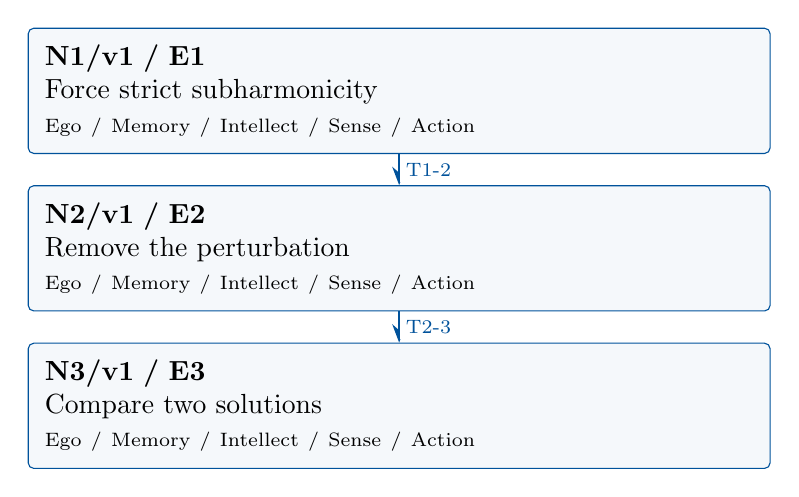
\begin{tikzpicture}[>=Stealth,x=1cm,y=1cm]

\node[mmnode,text width=9cm,minimum height=1.25cm] (N1) at (0,0.0) {\textbf{N1/v1 / E1}\\Force strict subharmonicity\\{\scriptsize Ego / Memory / Intellect / Sense / Action}};

\node[mmnode,text width=9cm,minimum height=1.25cm] (N2) at (0,-2.0) {\textbf{N2/v1 / E2}\\Remove the perturbation\\{\scriptsize Ego / Memory / Intellect / Sense / Action}};

\node[mmnode,text width=9cm,minimum height=1.25cm] (N3) at (0,-4.0) {\textbf{N3/v1 / E3}\\Compare two solutions\\{\scriptsize Ego / Memory / Intellect / Sense / Action}};

\draw[mmproof] (N1.south) -- node[mmnote,right] {T1-2} (N2.north);

\draw[mmproof] (N2.south) -- node[mmnote,right] {T2-3} (N3.north);

\end{tikzpicture}\end{center}

Each box is one mathematical agent containing all five faculties. Blue
arrows carry the versioned exports listed below. The layout gives a
reading order; only drawn arrows assert dependencies. Diagnostic repair
is separate from the proof DAG.

\subsection{Versioned evidence-transfer ledger}

\begingroup\small\linespread{1.05}\selectfont

\Needspace{5\baselineskip}\field{T1-2: N1/E1/v1 to N2}{\(\max_{\overline\Omega}u_\varepsilon=\max_{\partial\Omega}u_\varepsilon\).}

\field{Receiving activity}{N2.1}

\field{Compatibility}{E1/v1 and \(R^2=\max_{\overline\Omega}\|x\|^2<\infty\). Check: The error
bound must be independent of the point \(x\). Boundedness of the domain
provides that control.}

\Needspace{5\baselineskip}\field{T2-3: N2/E2/v1 to N3}{\(\max_{\overline\Omega}u=\max_{\partial\Omega}u\).}

\field{Receiving activity}{N3.1}

\field{Compatibility}{E2/v1 and \(u,v\) with equal Laplacians and equal boundary values in the
stated class. Check: Both signs are needed: one application gives only
one ordering.}

\endgroup

\clearpage\section{Agent roles and five-faculty activities}\begingroup\small\linespread{1.05}\selectfont\setlist{itemsep=1pt,topsep=2pt}

\subsection{N1/v1: Force strict subharmonicity}

\field{Object and role}{Use the positive Laplacian of the quadratic to contradict the
second-derivative test at an interior maximum. \textbf{Local
obligation:}
\(\max_{\overline\Omega}u_\varepsilon=\max_{\partial\Omega}u_\varepsilon\).}

\field{Inputs}{\(u_\varepsilon(x)=u(x)+\varepsilon\|x\|^2\) with \(\varepsilon>0\).}

\mmfaculty{E}{Ego}{Publish E1/v1 only after establishing this obligation:
\(\max_{\overline\Omega}u_\varepsilon=\max_{\partial\Omega}u_\varepsilon\).}

\mmfaculty{M}{Memory}{\(u_\varepsilon(x)=u(x)+\varepsilon\|x\|^2\) with \(\varepsilon>0\).
Retain the stated assumptions and import versions.}

\mmfaculty{I}{Intellect}{Use the positive Laplacian of the quadratic to contradict the
second-derivative test at an interior maximum.}

\mmfaculty{S}{Sense}{The maximum exists on the compact closure;
\(\Delta u_\varepsilon\ge2d\varepsilon>0\) rules out every interior
maximizing point.}

\mmfaculty{A}{Action}{Carry out activities N1.1--N1.2 below, retaining each calculation and
construction as evidence.}

\smallskip\noindent\textbf{Numbered mathematical activities}

\begin{enumerate}[label=N1.\arabic*,leftmargin=3.4em]

\item The perturbed function is continuous on the compact closure, so it
attains a maximum. At an interior maximum its Hessian has nonpositive
diagonal entries, giving \(\Delta u_\varepsilon\le0\).

\item But \(\Delta u_\varepsilon=\Delta u+2d\varepsilon>0\) everywhere inside.
Hence no maximizing point is interior; a maximizing point lies on the
boundary, proving the export.

\end{enumerate}

\field{Export E1/v1}{\(\max_{\overline\Omega}u_\varepsilon=\max_{\partial\Omega}u_\varepsilon\).}

\field{Acceptance gate}{The maximum exists on the compact closure;
\(\Delta u_\varepsilon\ge2d\varepsilon>0\) rules out every interior
maximizing point.}

\field{Targeted repair}{If \(\Delta u\ge0\) alone is claimed to contradict an interior maximum,
restore the strictly positive perturbation first. Withhold this export
and recheck its descendants after a versioned correction.}

\clearpage

\subsection{N2/v1: Remove the perturbation}

\field{Object and role}{Bound the perturbation uniformly so its effect vanishes as
\(\varepsilon\downarrow0\). \textbf{Local obligation:}
\(\max_{\overline\Omega}u=\max_{\partial\Omega}u\).}

\field{Inputs}{E1/v1 and \(R^2=\max_{\overline\Omega}\|x\|^2<\infty\). Incoming proof
exports: E1/v1 at N2.1.}

\mmfaculty{E}{Ego}{Publish E2/v1 only after establishing this obligation:
\(\max_{\overline\Omega}u=\max_{\partial\Omega}u\).}

\mmfaculty{M}{Memory}{E1/v1 and \(R^2=\max_{\overline\Omega}\|x\|^2<\infty\). Incoming proof
exports: E1/v1 at N2.1. Retain the stated assumptions and import
versions.}

\mmfaculty{I}{Intellect}{Bound the perturbation uniformly so its effect vanishes as
\(\varepsilon\downarrow0\).}

\mmfaculty{S}{Sense}{The error bound must be independent of the point \(x\). Boundedness of
the domain provides that control.}

\mmfaculty{A}{Action}{Carry out activities N2.1--N2.2 below, retaining each calculation and
construction as evidence.}

\smallskip\noindent\textbf{Numbered mathematical activities}

\begin{enumerate}[label=N2.\arabic*,leftmargin=3.4em]

\item For every \(x\in\overline\Omega\), E1 gives
\(u(x)\le u_\varepsilon(x)\le\max_{\partial\Omega}u+\varepsilon R^2\).
Let \(\varepsilon\downarrow0\) to obtain
\(u(x)\le\max_{\partial\Omega}u\).

\item Taking the maximum over the closure gives one inequality, and inclusion
of the boundary in the closure gives the reverse. This proves the
maximum principle.

\end{enumerate}

\field{Export E2/v1}{\(\max_{\overline\Omega}u=\max_{\partial\Omega}u\).}

\field{Acceptance gate}{The error bound must be independent of the point \(x\). Boundedness of
the domain provides that control.}

\field{Targeted repair}{If the quadratic perturbation is removed without a uniform bound, record
\(R\) before taking the limit. Withhold this export and recheck its
descendants after a versioned correction.}

\clearpage

\subsection{N3/v1: Compare two solutions}

\field{Object and role}{Apply the maximum principle to the difference and its negative.
\textbf{Local obligation:} \(u=v\) on \(\overline\Omega\), so the
classical Dirichlet problem has at most one solution in this class.}

\field{Inputs}{E2/v1 and \(u,v\) with equal Laplacians and equal boundary values in the
stated class. Incoming proof exports: E2/v1 at N3.1.}

\mmfaculty{E}{Ego}{Publish E3/v1 only after establishing this obligation: \(u=v\) on
\(\overline\Omega\), so the classical Dirichlet problem has at most one
solution in this class.}

\mmfaculty{M}{Memory}{E2/v1 and \(u,v\) with equal Laplacians and equal boundary values in the
stated class. Incoming proof exports: E2/v1 at N3.1. Retain the stated
assumptions and import versions.}

\mmfaculty{I}{Intellect}{Apply the maximum principle to the difference and its negative.}

\mmfaculty{S}{Sense}{Both signs are needed: one application gives only one ordering.}

\mmfaculty{A}{Action}{Carry out activities N3.1--N3.2 below, retaining each calculation and
construction as evidence.}

\smallskip\noindent\textbf{Numbered mathematical activities}

\begin{enumerate}[label=N3.\arabic*,leftmargin=3.4em]

\item The difference \(w=u-v\) has \(\Delta w=0\) and zero boundary values.
Apply E2 to \(w\) to get \(w\le0\).

\item Apply it to \(-w\), whose Laplacian also vanishes, to get \(-w\le0\).
Thus \(w=0\). This proves uniqueness without asserting existence for
arbitrary data.

\end{enumerate}

\field{Export E3/v1}{\(u=v\) on \(\overline\Omega\), so the classical Dirichlet problem has
at most one solution in this class.}

\field{Acceptance gate}{Both signs are needed: one application gives only one ordering.}

\field{Targeted repair}{If uniqueness is inferred from only \(w\le0\), apply the same argument
to \(-w\) before exporting equality. Withhold this export and recheck
its descendants after a versioned correction.}

\endgroup\clearpage\section{Continuous mathematical proof}\label{sec:proof}

\subsection{N1 --- Force strict
subharmonicity}\label{n1-force-strict-subharmonicity}

\begin{enumerate}
\def\labelenumi{\arabic{enumi}.}
\item
  \textbf{N1.1.} The perturbed function is continuous on the compact
  closure, so it attains a maximum. At an interior maximum its Hessian
  has nonpositive diagonal entries, giving \(\Delta u_\varepsilon\le0\).
\item
  \textbf{N1.2.} But \(\Delta u_\varepsilon=\Delta u+2d\varepsilon>0\)
  everywhere inside. Hence no maximizing point is interior; a maximizing
  point lies on the boundary, proving the export.
\end{enumerate}

\subsection{N2 --- Remove the
perturbation}\label{n2-remove-the-perturbation}

\begin{enumerate}
\def\labelenumi{\arabic{enumi}.}
\item
  \textbf{N2.1.} For every \(x\in\overline\Omega\), E1 gives
  \(u(x)\le u_\varepsilon(x)\le\max_{\partial\Omega}u+\varepsilon R^2\).
  Let \(\varepsilon\downarrow0\) to obtain
  \(u(x)\le\max_{\partial\Omega}u\).
\item
  \textbf{N2.2.} Taking the maximum over the closure gives one
  inequality, and inclusion of the boundary in the closure gives the
  reverse. This proves the maximum principle.
\end{enumerate}

\subsection{N3 --- Compare two
solutions}\label{n3-compare-two-solutions}

\begin{enumerate}
\def\labelenumi{\arabic{enumi}.}
\item
  \textbf{N3.1.} The difference \(w=u-v\) has \(\Delta w=0\) and zero
  boundary values. Apply E2 to \(w\) to get \(w\le0\).
\item
  \textbf{N3.2.} Apply it to \(-w\), whose Laplacian also vanishes, to
  get \(-w\le0\). Thus \(w=0\). This proves uniqueness without asserting
  existence for arbitrary data.
\end{enumerate}

\hfill$\square$

\section{Worked orchestration}

On the unit disk in \(\mathbb R^2\), \(u(x,y)=x^2+y^2\) has
\(\Delta u=4\) and maximum one on the boundary. For harmonic boundary
data given by the restriction of \(x\), the function \(u(x,y)=x\) is a
solution, and the comparison argument proves it is the only one in the
stated class.

\subsection{Boundary and hypothesis audit}

Boundedness cannot simply be dropped. On the upper half-plane,
\(u(x,y)=y\) is harmonic and continuous up to the boundary, where it is
zero, but it is positive and unbounded inside. Compact maximum
attainment and the uniform perturbation bound both fail.

\section{Illustrative failure and repair}

The following is an authored diagnostic scenario. Changed assumptions
define a new contract; they do not retroactively prove the original
statement.

\subsection{Rejected argument, diagnosis, and correction}
\textbf{Rejected N1 argument:} an interior maximum contradicts
\(\Delta u\ge0\). A constant function has interior maxima and
\(\Delta u=0\), so the claimed contradiction is invalid.
\textbf{Repair:} use \(u_\varepsilon\) to obtain strict positivity,
prove boundary attainment there, and then remove the perturbation. This
fixes the proof while leaving the target weak maximum principle
unchanged; recheck E2 and the uniqueness corollary.

\subsection{Publication and reuse}
The corrected export retains its explicit assumptions. A hypothetical
revision receives a new version, and each consuming activity is
rechecked; this scenario is not a recorded runtime event. \textbf{Next
direction:} Develop comparison for nonzero forcing or the strong maximum
principle with its additional connectedness and argument.

\par\medskip\begingroup\small\linespread{1.0}\selectfont\noindent\textbf{Provenance.} This authored proof is complete relative to its declared imports. Reuse
each export with its assumptions, proof, and version. The original
Markdown remains available for comparison.
\par\endgroup

\par\smallskip\begingroup\small\linespread{1.0}\selectfont\noindent\textbf{Further reading.} \href{https://math.stanford.edu/~lms/lecs-on-pde.pdf}{Leon Simon,
Lectures on PDE}, for elliptic, weak, and parabolic methods. Classical
calculus and the explicitly stated Hilbert-space imports are used below;
the displayed PDE arguments are developed in full.\par\endgroup

\end{document}
